\documentclass{beamer}
\usetheme{Boadilla}

\title{My Beamer Presentation}
\subtitle{Having a great time}
\author{Andrew Dunn}
\institute{Central Washington University}
\date{\today}

\begin{document}
    \begin{frame}
        \titlepage
    \end{frame}
    
    \begin{frame}
        \frametitle{Outline}
        \tableofcontents
    \end{frame}
    
    \section{Section 1}
    \subsection{sub a}
     
    \begin{frame}
        \frametitle{Title}
        Hey look, it's a \alert{title}
    \end{frame}
    
    \begin{frame}
        \frametitle{List}
        \begin{itemize}
            \item Point A
            \item Point B
            \begin{itemize}
                \item part 1
                \item part 2
            \end{itemize}
            \item Point C
            \item Point D
        \end{itemize}
    \end{frame}
    
    \begin{frame}
        \begin{description}
            \item[API] Application Programming Interface
            \item[LAN] Local Area Network
            \item[ASCII] American Standard Code for Information Interchange
        \end{description}
    \end{frame}
    
    \begin{frame}[fragile]
        \frametitle{Including Code}
        \begin{semiverbatim}
            \\begin\{frame\}
            \\frametitle\{Outline\}
            \\tableofcontents
            \\end\{frame\}
        \end{semiverbatim}
    \end{frame}
    
    \begin{frame}{Slide "pauses"}
        \begin{itemize}
            \item First Point
                \pause
            \item Second Point
                \pause
            \item Third Point
        \end{itemize}
    \end{frame}
    
    \begin{frame}{Columns}
        \begin{columns}
            \column{0.5\textwidth}
            \begin{align*}
                f(x) = x^2
            \end{align*}
            \column{0.5\textwidth}
            \begin{align*}
                h(x) &= \frac{1}{x} \\
                w(x) &= \int^a_b \frac{1}{2}x^3 \\
                m(x) &= \frac{1}{\sqrt{x^3}}
            \end{align*}
        \end{columns}
    \end{frame}
    
    \begin{frame}{Picture in columns}
        \begin{columns}
            \column{0.5\textwidth}
            \centering
            Hey look over there, it's a dog!
            \column{0.5\textwidth}
            \centering
            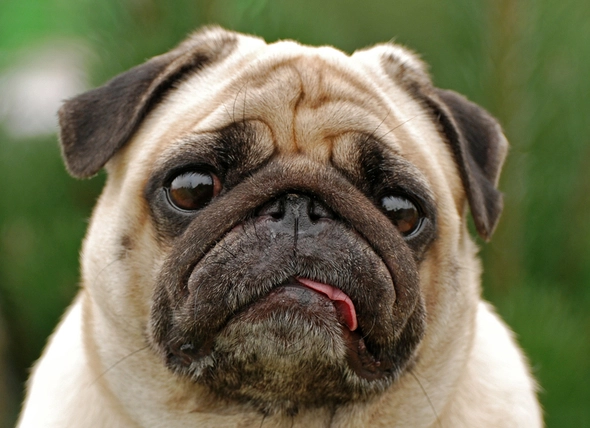
\includegraphics[scale=0.3]{pug.png}
        \end{columns}
    \end{frame}
    
    \begin{frame}{Blocks}
        \begin{block}{A question}
            And an answer
        \end{block}
        \begin{block}{Another question}
            And another answer
        \end{block}
    \end{frame}
    
\end{document}